\section{Background}
\label{sec:background}

\subsection{The Problem}
\label{subsec:the_problem}

Throughout Sqlite's history many tests, papers, and tools have been developed in order to understand, and modify the future direction of Sqlite. However, when a user wants to understand at a deeper level how Sqlite is working or finding obscure bugs, they are stuck with manually trawling through a Hex editor. This paper aims to solve this by providing a visualisation of the internal structure, as well as a update log that is updated in real time, when the database is modified.


\subsection{Sqlite}
\label{subsec:sqlite}

\subsubsection{What is Sqlite}
\label{subsubsec:what_is_sqlite}

Sqlite is a single self-contained, serverless SQL database engine. Started on 29 May 2000 by D. Richard Hipp \citep{sqlite} from gathered inspiration while working on software for guided missiles on a battleship where they needed a self-contained portable database. \citep{sqlitedefguide} He joined up with Joe Mistachkin followed by Dan Kennedy in 2002. Version 1.0 was released in August 2000, then in just over year on the 28 November 2001 2.0 which introduced, BTrees and many of the features seen in 3.0. Which came a lot later containing a full rewrite and improvement over 2.0, with the first public release on 18 June 2004. At the time of writing this paper we are currently sitting at version 3.10.4 \citep{sqlite}.
\\\\
Sqlite is open source within the public domain making it accessible to everyone. The entire library size can be 350Kib, with some option features omitted it could be reduced to around 300Kib making it incredibly small compared to what it does. In addition to this the runtime usage is minimal with 4Kib stack space and 100Kib heap, allowing it to run on almost anything. Sqlite's main strength is that the entire database in encoded into a single portable file, that can be read, on any system whether 32 or 64 bit, big or small endian. It is often seen as a replacement for storage files rather then a database system \citep{sqlite}.

\subsubsection{Where is Sqlite used}
\label{subsubsec:where_is_sqlite}

As Sqlite is a minimal portable database engine it has primarily two uses, The first as a relation database like any other, the second as a application file format. In the former case Sqlite would be set up the same way a tradition database system would be, with the primary purpose to hold the back end storage information. The latter case is more unique to Sqlite and is what sets it apart from the traditional database engines \citep{sqlite}. Because of this Sqlite is used everywhere, a few of the big names include, apple, android, adobe even a special version was produced specifically for windows 10. In fact Sqlite might be the single most deployed software currently \citep{sqlite, sqlitetalk}.

\subsubsection{How is Sqlite works}
\label{subsubsec:how_sqlite_works}

Sqlite consist of three main parts, the backend, core and the SQL compiler. Figure~\ref{fig:sqlite_arch} shows the architectural digram of Sqlite.

\begin{figure}[h]
	\centering
	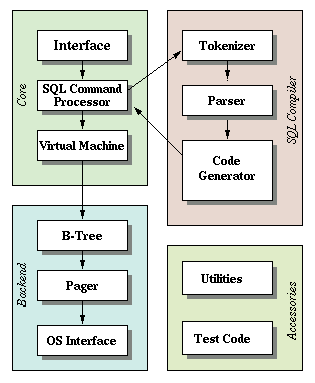
\includegraphics[scale=0.5]{images/sqlite_arch.png}
	\caption{Sqlite architectural diagram \citep{sqlite}}
	\label{fig:sqlite_arch}
\end{figure}

The SQL compiler is designed to take SQL strings and turn them into valid SQL commands, it is made up of three parts. Firstly the tokenizer takes a string containing SQL statements and turns it into tokens passing them one bay one to the parser. The parser takes the tokens and assign meaning to them. Lastly the code generator takes the tokens from the parser and assembles complete SQL statements that are to be ran on the database file.
\\\\
The Core itself is actually a virtual machine implementing a specifically designed computing engine to manipulate database files. The interface module defines the interface between the virtual machine and the SQL library including the external API. Knowing this we can see that the virtual machine takes the code output from the code generator to manipulate the backend / database. 
\\\\
The final main module is the backend which is the main focus of this paper, controlling the file format. The OS interface contains an abstraction layer to write the files to disk or memory. The Pager takes the B-Trees and is responsible for reading, writing and caching them. This involves locking, rollback and atomic commits of the database. Sqlite uses a B-Tree system to navigate and store the data on disk, this module contains the implementation of the B-tree and as such the defines the file format. 
\\\\
The last module, accessories is made up of two parts. Utilities contain functions that are used all around Sqlite, such as memory allocation, string comparison, random number generator and symbol tables. The test section contains all the test scripts and only exist for testing purposes, of which contains over 811 times more code then the actual project.

\subsection{The Sqlite file format}
\label{subsec:sqlite_file_format}

\subsubsection{The page system}
\label{subsubsec:sqlite_page_system}

Sqlite is made up of pages..

\subsubsection{The Trees and Cells}
\label{subsubsec:sqlite_trees_and_cells}

The Trees and cells...

\subsubsection{Encoding of the data}
\label{subsubsec:sqlite_data_encoding}

The Data is...

\subsection{Similar Programs}
\label{subsec:similar_programs}

\subsubsection{Sqlite browser}
\label{subsubsec:sqlite_browser}

One Similar program...